% file: hoare-partition-example.tex
% an array of length 11 

\documentclass[tikz]{standalone}
\usetikzlibrary{decorations.pathreplacing, positioning, arrows.meta, shapes.multipart, calc}

\begin{document}
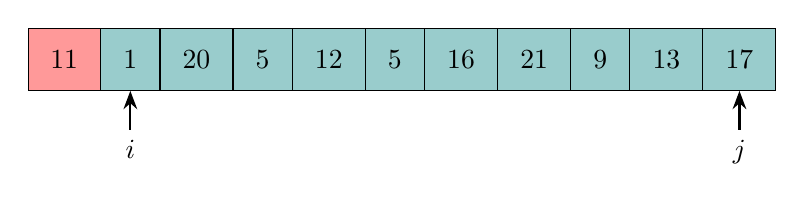
\begin{tikzpicture}[Array/.style = {rectangle split, rectangle split parts = #1, rectangle split horizontal,
    inner sep = 8pt, anchor = center}]
  \node[Array = {11}, draw, rectangle split part fill = {red!40, teal!40}] (A) 
    {11\nodepart{two}1\nodepart{three}20\nodepart{four}5\nodepart{five}12\nodepart{six}5\nodepart{seven}16\nodepart{eight}21\nodepart{nine}9
    \nodepart{ten}13\nodepart{eleven}17};

    \draw[<-, >=Stealth, thick] (A.two south) -- ($(A.two south) + (0, -0.5cm)$) node[below] {$i$};
    \draw[<-, >=Stealth, thick] (A.eleven south) -- ($(A.eleven south) + (0, -0.5cm)$) node[below] {$j$};
\end{tikzpicture}
\end{document}
